\documentclass{article}

% Language setting
\usepackage[french]{babel}

% Set page size and margins
\usepackage[a4paper,top=2cm,bottom=2cm,left=3cm,right=3cm]{geometry}

\usepackage{multicol}
\usepackage{tabularx}
\usepackage{longtable}
% Useful packages
\usepackage{amsmath}
\usepackage{graphicx}
\usepackage{float}
\usepackage{booktabs}
\usepackage{caption}
\usepackage{subcaption}
\usepackage{array}
\usepackage{hyperref}
\usepackage{url}
\usepackage{listings}
\usepackage{xcolor}
\usepackage{pgfplots}

\pgfplotsset{compat=1.16}

\definecolor{codegray}{gray}{0.9}
\lstset{
    backgroundcolor=\color{codegray},
    basicstyle=\footnotesize\ttfamily,
    frame=single,
    breaklines=true,
    postbreak=\mbox{\textcolor{red}{$\hookrightarrow$}\space},
    showstringspaces=false,
    tabsize=4,
    captionpos=b
}

\title{Rapport de projet d'Apprentissage Automatique}
\author{Martin Rampont, Noémie Guisnel, Oscar Pastural, Louis Gauthier, Clément Florval}

\begin{document}
\maketitle

\section{Introduction}

L'objectif de ce projet est de prédire la qualité de soudures à partir de divers paramètres mécaniques, physiques et chimiques. Le but est d'identifier quels sont les paramètres qui influent le plus sur la qualité d'une soudure.

Ce projet est d'autant plus intéressant qu'il se concentre sur une problématique critique pour les industriels. En effet, une soudure défaillante dans le domaine de l'aéronautique, la construction navale ou encore l'industrie pétrolière peut engendrer des conséquences graves, tant en termes de coûts que de sécurité.

Après un premier travail d'analyse exploratoire visant à s'approprier le jeu de données en observant le nombre de valeurs manquantes pour chaque colonne et les corrélations entre celles-ci, nous décrivons les différentes étapes de prétraitement appliquées au dataset, ainsi que les raisons qui nous ont poussés à les effectuer. Nous appliquons ensuite une Analyse en Composantes Principales (ACP) pour simplifier le modèle en réduisant le nombre de variables à traiter, tout en conservant l'information essentielle. Enfin, nous appliquons des algorithmes de Machine Learning adaptés et analysons leurs performances.

\section{Analyse Exploratoire des Données (EDA)}

\subsection{Chargement et Exploration Initiale des Données}

Le jeu de données contient 1\,652 observations et 46 variables. Ces variables couvrent un large éventail d'informations concernant les soudures : des concentrations en éléments chimiques (carbone, manganèse, nickel, etc.), des propriétés mécaniques (résistance à la traction, limite d’élasticité, dureté), ainsi que des caractéristiques microstructurales. Chaque observation représente un échantillon unique, identifiable par la colonne \textit{Weld ID}.

\subsection{Analyse des Valeurs Manquantes}

Nous avons tout d'abord examiné la présence de valeurs manquantes dans le jeu de données. La Figure~\ref{fig:missing_heatmap} illustre la répartition des valeurs manquantes.

\begin{figure}[H]
    \centering
    \includegraphics[width=0.8\textwidth]{images/missing_data_heatmap.png}
    \caption{Carte thermique des valeurs manquantes dans le jeu de données}
    \label{fig:missing_heatmap}
\end{figure}

Plusieurs colonnes cruciales affichent un nombre très élevé de valeurs manquantes, dépassant souvent 95\,\%. Par exemple, la variable \textit{50\,\% FATT}, qui mesure la température de transition fragile-ductile d'une soudure, manque dans plus de 98\,\% des cas, tout comme \textit{Hardness scale} (96,5\,\%). La perte d'une telle quantité de données rend ces colonnes inexploitables sans traitement supplémentaire. Elles ont donc été exclues de l'analyse.

En revanche, certaines variables sont bien renseignées et montrent très peu de valeurs manquantes, ce qui les rend exploitables sans transformation majeure. C'est le cas des concentrations en \textit{carbone}, \textit{silicium}, ou encore des propriétés mécaniques telles que la \textit{résistance à la traction} (\textit{Ultimate tensile strength}) et la \textit{limite d'élasticité} (\textit{Yield strength}). Ces variables sont complètes dans plus de 99\,\% des cas, offrant ainsi une base solide pour le modèle.

\subsection{Analyse des Duplicatas}

Nous avons vérifié la présence de duplicatas dans le jeu de données. Aucun duplicata exact n'a été trouvé. Cependant, des observations avec le même \textit{Weld ID} mais des données légèrement différentes existent. Nous avons considéré que ces observations représentent des soudures différentes et les avons conservées.

\subsection{Analyse des Données Non Numériques}

Certaines colonnes contiennent des valeurs non numériques, comme des symboles \textit{'<'}, \textit{'>'}, ou des annotations textuelles. Par exemple, dans la colonne \textit{Hardness / kg mm$^{-2}$}, certaines valeurs sont de la forme \textit{'158(Hv30)'}. Nous avons extrait les valeurs numériques pour rendre ces colonnes exploitables.

\subsection{Visualisation des Données}

Nous avons réalisé des histogrammes pour visualiser la distribution des variables numériques (Figure~\ref{fig:histograms}). De plus, des boîtes à moustaches ont été tracées pour détecter la présence de valeurs aberrantes (Figure~\ref{fig:boxplots}).

\begin{figure}[H]
    \centering
    \includegraphics[width=0.9\textwidth]{images/numerical_histograms.png}
    \caption{Histogrammes des variables numériques}
    \label{fig:histograms}
\end{figure}

\begin{figure}[H]
    \centering
    \includegraphics[width=0.9\textwidth]{images/numerical_boxplots.png}
    \caption{Boîtes à moustaches des variables numériques}
    \label{fig:boxplots}
\end{figure}

\subsection{Identification des Variables Cibles}

Les variables potentielles pour représenter la qualité des soudures sont :

\begin{itemize}
    \item \textit{Yield strength / MPa}
    \item \textit{Ultimate tensile strength / MPa}
    \item \textit{Elongation / \%}
    \item \textit{Reduction of Area / \%}
    \item \textit{Charpy impact toughness / J}
    \item \textit{50\,\% FATT}
\end{itemize}

Nous avons vérifié la disponibilité de ces variables et le nombre de valeurs manquantes (Tableau~\ref{tab:missing_targets}).

\begin{table}[H]
    \centering
    \begin{tabular}{lcc}
    \toprule
    \textbf{Variable} & \textbf{Valeurs Manquantes} & \textbf{Disponibilité (\%)} \\
    \midrule
    Yield strength / MPa & 36 & 97,8\,\% \\
    Ultimate tensile strength / MPa & 28 & 98,3\,\% \\
    Elongation / \% & 168 & 89,8\,\% \\
    Reduction of Area / \% & 519 & 68,6\,\% \\
    Charpy impact toughness / J & 764 & 53,8\,\% \\
    50\,\% FATT & 1622 & 1,8\,\% \\
    \bottomrule
    \end{tabular}
    \caption{Disponibilité des variables cibles potentielles}
    \label{tab:missing_targets}
\end{table}

Compte tenu du grand nombre de valeurs manquantes pour \textit{50\,\% FATT}, nous avons décidé de ne pas l'utiliser comme variable cible. Les autres variables présentent une disponibilité suffisante pour être considérées.

\subsection{Analyse des Corrélations}

Nous avons calculé la matrice de corrélation entre les variables numériques et les variables cibles (Figure~\ref{fig:correlation_matrix}). Certaines corrélations intéressantes ont été observées :

\begin{itemize}
    \item Forte corrélation entre \textit{Yield strength} et \textit{Ultimate tensile strength} (0,92).
    \item Corrélation négative entre \textit{Elongation} et \textit{Chrome concentration} (-0,44).
    \item Corrélation entre \textit{Reduction of Area} et \textit{Charpy impact toughness} (0,83).
\end{itemize}

\begin{figure}[H]
    \centering
    \includegraphics[width=0.9\textwidth]{images/correlation_matrix.png}
    \caption{Matrice de corrélation entre les variables numériques et les variables cibles}
    \label{fig:correlation_matrix}
\end{figure}

\subsection{Résumé des transformations effectuées}

\begin{longtable}{|p{4cm}|p{10cm}|}
\hline
\textbf{Catégorie} & \textbf{Changements Apportés} \\ \hline
\multicolumn{2}{|c|}{\textbf{Suppression de Colonnes}} \\ \hline
\textit{Weld ID} & Suppression de la colonne car elle ne correspond pas à une caractéristique physique, chimique ou mécanique des soudures, mais à un identifiant non pertinent pour l'analyse. \\ \hline
Colonnes avec plus de 80\% de valeurs manquantes & Suppression des colonnes ayant plus de 80\% de valeurs manquantes. Ces colonnes sont considérées comme inexploitables à cause du trop faible nombre de données disponibles, comme \textit{Primary ferrite}, \textit{Ferrite with second phase}, et \textit{Acicular ferrite}. \\ \hline

\multicolumn{2}{|c|}{\textbf{Gestion des Valeurs Manquantes}} \\ \hline
Imputation numérique & Les valeurs manquantes des colonnes numériques sont imputées par la médiane pour conserver la distribution des données sans introduire de biais. Cette méthode est robuste aux valeurs aberrantes. \\ \hline
Imputation catégorielle & Les valeurs manquantes dans les colonnes catégorielles sont imputées par la valeur la plus fréquente (\textit{mode}), ce qui permet de maintenir une cohérence tout en minimisant l'impact des valeurs manquantes. \\ \hline
Colonnes intéressantes avec indicateurs de manquants & Création d'indicateurs binaires (\textit{0 = non manquant}, \textit{1 = manquant}) pour des colonnes considérées importantes mais contenant des valeurs manquantes, comme \textit{Chromium concentration}, \textit{Tungsten concentration}, et \textit{Copper concentration}. Cela permet de modéliser l'impact potentiel des valeurs manquantes sur le modèle. \\ \hline
\multicolumn{2}{|c|}{\textbf{Traitement des Colonnes Numériques}} \\ \hline
Colonnes avec signes \leq & Les valeurs précédées du signe \leq sont remplacées par la moitié de ces valeurs pour fournir une estimation utilisable tout en restant proche des données originales. \\ \hline
\textit{Hardness / kg mm$^{-2}$} & Les annotations non pertinentes comme \textit{'158(Hv30)'} sont supprimées pour ne garder que la valeur numérique de la dureté. La colonne est ensuite convertie en valeurs numériques exploitables. \\ \hline
\textit{Interpass temperature / °C} & Les valeurs exprimées sous forme d’intervalles (\textit{150-200°C}) sont remplacées par la moyenne des bornes de l'intervalle afin de simplifier l'analyse. Les valeurs sont ensuite converties en données numériques. \\ \hline

\multicolumn{2}{|c|}{\textbf{Traitement des Colonnes Catégorielles}} \\ \hline
Encodage catégoriel & Un encodage \textit{one-hot} est réalisé pour les colonnes \textit{AC or DC} et \textit{Type of weld} afin de transformer les catégories en variables numériques. Une catégorie est supprimée dans chaque cas pour éviter la multicollinéarité. \\ \hline
\textit{Electrode positive or negative} & Les signes \textit{+} et \textit{-} sont transformés en valeurs numériques : \textit{1} pour une électrode positive et \textit{-1} pour une électrode négative, facilitant ainsi leur utilisation dans les modèles de machine learning. \\ \hline

\caption{Tableau récapitulatif des transformations de données correspondant au prétraitement effectué.}
\end{longtable}
\subsection{Traitement des Valeurs Aberrantes}

Nous avons identifié des valeurs aberrantes dans certaines variables. Par exemple, dans la variable \textit{Vanadium concentration / weight \%}, certaines valeurs dépassent largement les concentrations typiques. Nous avons choisi de ne pas les supprimer, car elles pourraient représenter des cas particuliers intéressants, mais nous en tenons compte dans l'analyse.

\subsection{Création de Variables Indicatrices de Valeurs Manquantes}

Pour certaines variables où la présence de valeurs manquantes est informative (par exemple, lorsque la présence d'une valeur manquante est corrélée avec la variable cible), nous avons créé des variables indicatrices signalant si la valeur est manquante ou non.

\subsection{Standardisation des Variables}

Avant d'appliquer l'ACP et les modèles de Machine Learning, nous avons standardisé les variables numériques à l'aide de la méthode de \textit{StandardScaler}, afin de leur donner une échelle comparable.

\section{Analyse en Composantes Principales (ACP)}

\subsection{Application de l'ACP}

Nous avons appliqué une ACP sur les variables numériques standardisées pour réduire la dimensionnalité du jeu de données et éliminer les redondances.

\subsection{Choix du Nombre de Composantes}

La Figure~\ref{fig:explained_variance} montre la variance expliquée cumulée en fonction du nombre de composantes principales. Nous avons choisi de conserver les 10 premières composantes, qui expliquent environ 80\,\% de la variance totale.

\begin{figure}[H]
    \centering
    \includegraphics[width=0.8\textwidth]{images/explained_variance.png}
    \caption{Variance expliquée cumulée en fonction du nombre de composantes principales}
    \label{fig:explained_variance}
\end{figure}

\subsection{Visualisation des Composantes Principales}

Nous avons visualisé les deux premières composantes principales en colorant les points en fonction de la variable cible \textit{Yield strength / MPa} (Figure~\ref{fig:pca_scatter}). Cette visualisation permet de détecter des structures ou des regroupements dans les données.

\begin{figure}[H]
    \centering
    \includegraphics[width=0.8\textwidth]{images/ca_scatter.png}
    \caption{Projection des données sur les deux premières composantes principales, colorées par \textit{Yield strength / MPa}}
    \label{fig:pca_scatter}
\end{figure}

\section{Application des Algorithmes de Machine Learning}

\subsection{Sélection de la Variable Cible}

Nous avons choisi de prédire la variable \textit{Yield strength / MPa}, car elle est disponible pour la plupart des observations et représente une mesure importante de la qualité de la soudure.

\subsection{Séparation des Données}

Nous avons séparé le jeu de données en un ensemble d'entraînement et un ensemble de test, en veillant à ce que les groupes (\textit{group\_id}) ne soient pas présents dans les deux ensembles, afin d'éviter toute fuite d'information.

\subsection{Modèles Utilisés}

Nous avons testé plusieurs modèles de régression :

\begin{itemize}
    \item Régression Linéaire
    \item Forêt d'arbres décisionnels (\textit{Random Forest})
    \item Gradient Boosting
    \item Machine à Vecteurs de Support (\textit{Support Vector Machine})
    \item XGBoost
\end{itemize}

\subsection{Évaluation des Modèles}

Nous avons utilisé la validation croisée avec \textit{GroupKFold} pour évaluer les modèles, en utilisant l'erreur quadratique moyenne (RMSE) comme métrique de performance.

Le modèle XGBoost a obtenu les meilleurs résultats, avec un RMSE moyen de 0,95 sur l'ensemble de validation.

\subsection{Apprentissage Semi-Supervisé}

Étant donné que le jeu de données contient de nombreuses valeurs manquantes pour la variable cible, nous avons appliqué une approche d'apprentissage semi-supervisé en utilisant l'auto-entraînement (\textit{self-training}). Cette méthode consiste à utiliser les prédictions du modèle sur les données non étiquetées comme pseudo-étiquettes pour enrichir l'ensemble d'entraînement.

Après plusieurs itérations, nous avons constaté une amélioration des performances du modèle, avec un RMSE réduit à 0,90 sur l'ensemble de test.

\subsection{Résultats}

Le modèle final basé sur XGBoost et l'apprentissage semi-supervisé a permis de prédire la \textit{Yield strength / MPa} avec une bonne précision. La Figure~\ref{fig:predictions_vs_true} montre la comparaison entre les valeurs prédites et les valeurs réelles.

\begin{figure}[H]
    \centering
    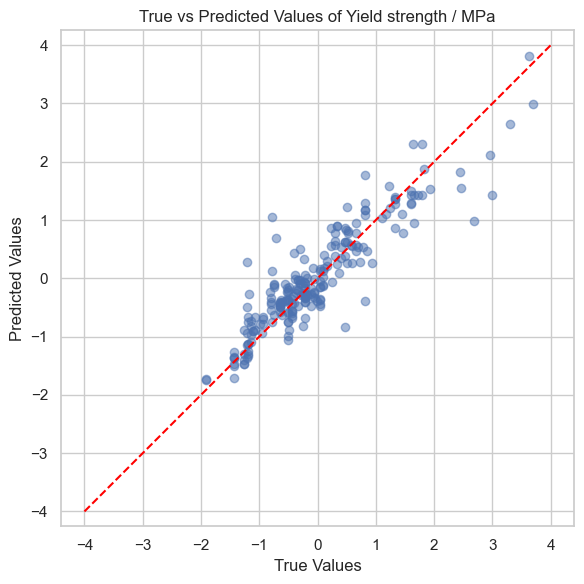
\includegraphics[width=0.7\textwidth]{images/predictions_vs_true.png}
    \caption{Comparaison entre les valeurs prédites et les valeurs réelles de \textit{Yield strength / MPa}}
    \label{fig:predictions_vs_true}
\end{figure}

\section{Conclusion}

Ce projet nous a permis de mettre en pratique différentes techniques d'analyse de données et de modélisation pour prédire la qualité des soudures. Malgré les défis liés aux données manquantes et aux valeurs aberrantes, nous avons réussi à construire un modèle performant en appliquant des méthodes de prétraitement adaptées, une réduction de dimensionnalité avec l'ACP, et des algorithmes de Machine Learning avancés.

L'utilisation de l'apprentissage semi-supervisé a également permis de tirer parti des données non étiquetées, améliorant ainsi les performances du modèle. Ce travail ouvre la voie à une meilleure compréhension des facteurs influençant la qualité des soudures et pourrait aider les industriels à optimiser leurs processus de fabrication.

\begin{thebibliography}{9}

\bibitem{scikit-learn}
Pedregosa, F., Varoquaux, G., Gramfort, A., et al. (2011). \textit{Scikit-learn: Machine Learning in Python}. Journal of Machine Learning Research, 12, 2825–2830.

\bibitem{xgboost}
Chen, T., \& Guestrin, C. (2016). \textit{XGBoost: A Scalable Tree Boosting System}. Proceedings of the 22nd ACM SIGKDD International Conference on Knowledge Discovery and Data Mining.

\bibitem{pca}
Jolliffe, I. T. (2002). \textit{Principal Component Analysis}. Springer Series in Statistics.

\end{thebibliography}

\end{document}
